% Adjust these for the path of the theme and its graphics, relative to this file
%\usepackage{beamerthemeFalmouthGamesAcademy}
\usepackage{../../beamerthemeFalmouthGamesAcademy}
\usepackage{multimedia}
\graphicspath{ {../../} }

% Default language for code listings
\lstset{language=Python
}

% For strikethrough effect
\usepackage[normalem]{ulem}
\usepackage{wasysym}

\usepackage{algpseudocode}

\usepackage{pdfpages}
\usepackage{qtree}

% http://www.texample.net/tikz/examples/state-machine/
\usetikzlibrary{arrows,automata}
\usetikzlibrary{tikzmark,calc}

\newcommand{\modulecode}{COMP140 GAM160}\newcommand{\moduletitle}{Hacking Hardware/Advanced Programming}\newcommand{\sessionnumber}{Session 6}

\begin{document}
\title{\sessionnumber: Data Structures I}
\subtitle{\modulecode: \moduletitle}

\frame{\titlepage} 

%\begin{frame}
%	\frametitle{Learning outcomes}
%	\begin{itemize}
%		\item \textbf{Explain} the difference between pass-by-value and pass-by-reference
%		\item \textbf{Distinguish} the basic data structures available in Python
%		\item \textbf{Determine} the complexity of accessing and manipulating data in these data structures
%		\item \textbf{Choose} the correct data structure for a given task
%	\end{itemize}
%\end{frame}

\begin{frame}{Assignments}
	\begin{itemize}
		\item Peer review \textbf{next Thursday}
		\item Please come to the session with a \textbf{draft} of your research journal
	\end{itemize}
	\vspace{3ex}
	\begin{itemize}
		\item Worksheet 5 due \textbf{tomorrow}
		\item \textbf{No new worksheet} this week --- work on your research journal instead
	\end{itemize}
\end{frame}

\part{Turing machines}
\frame{\partpage}

\begin{frame}{Turing machines}
    \begin{itemize}
        \pause\item Introduced in 1936 by Alan Turing
        \pause\item Theoretical model of a ``computer''
            \begin{itemize}
                \pause\item I.e.\ a machine that carries out computations (calculations)
            \end{itemize}
    \end{itemize}
\end{frame}

\begin{frame}{Turing machine}
    \begin{itemize}
        \pause\item Has a finite number of \textbf{states}
        \pause\item Has an infinite \textbf{tape}
        \pause\item Each space on the tape holds a \textbf{symbol} from a finite \textbf{alphabet}
        \pause\item Has a \textbf{tape head} pointing at one space on the tape
        \pause\item Has a transition table which, given:
            \begin{itemize}
                \item The current state
                \item The symbol under the tape head
            \end{itemize}
        specifies:
            \begin{itemize}
                \item A new state
                \item A new symbol to write to the tape, overwriting the current symbol
                \item Where to move the tape head: one space to the left, or one space to the right
            \end{itemize}
    \end{itemize}
\end{frame}

\newcommand{\stateA}{Drumstick}
\newcommand{\stateB}{Fruit}
\newcommand{\stateC}{Swizzels}
\newcommand{\tapeX}{Blank}
\newcommand{\tapeO}{Milk}
\newcommand{\tapeI}{White}

\begin{frame}{Activity}
    \begin{itemize}
        \pause\item In groups of 3-4
        \pause\item Line up 5-10 chocolates of different colours --- this is your \textbf{tape}
        \pause\item Point your \textbf{\stateA} lolly at the \textbf{leftmost} chocolate
            \begin{itemize}
                \pause\item The lolly is your \textbf{tape head}, and the type of lolly is your \textbf{state}
            \end{itemize}
        \pause\item Repeatedly apply the rules on the next slide
        \pause\item What computation does this machine perform?
            \begin{itemize}
                \pause\item Hint: $\text{\tapeO}=0$, $\text{\tapeI}=1$...
            \end{itemize}
    \end{itemize}
\end{frame}

\begin{frame}
    \begin{tabular}{|cc|ccc|} \hline
        Current & Current & New & New & Move \\
        lolly & chocolate & lolly & chocolate & direction \\\hline
        \stateA & \tapeX & \stateB & \tapeX & $\leftarrow$  \\
        \stateA & \tapeO & \stateA & \tapeI & $\rightarrow$ \\
        \stateA & \tapeI & \stateA & \tapeO & $\rightarrow$ \\\hline
        \stateB & \tapeX & \stateC & \tapeI & $\rightarrow$ \\
        \stateB & \tapeO & \stateC & \tapeI & $\leftarrow$  \\
        \stateB & \tapeI & \stateB & \tapeO & $\leftarrow$  \\\hline
        \stateC & \tapeX & Stop    & \tapeX & $\rightarrow$ \\
        \stateC & \tapeO & \stateC & \tapeO & $\leftarrow$  \\
        \stateC & \tapeI & \stateC & \tapeI & $\leftarrow$  \\\hline
    \end{tabular}
\end{frame}

\begin{frame}{The Church-Turing Thesis}
    \begin{itemize}
        \pause\item If a calculation can be carried out by a mechanical process at all,
            then it can be carried out by a Turing machine
        \pause\item I.e.\ a Turing machine is the most ``powerful'' computer possible,
            in terms of what is possible or impossible to compute
        \pause\item A machine, language or system is \textbf{Turing complete} if it can simulate a Turing machine
    \end{itemize}
\end{frame}


\part{Computability}
\frame{\partpage}

\begin{frame}{Computability theory}
	\begin{itemize}
		\pause\item Let $A$ and $B$ be \textbf{sets} of elements
			\begin{itemize}
				\pause\item NB: $A$ may be \textbf{infinite}
			\end{itemize}
		\pause\item A function $f : A \to B$ is \textbf{computable} if there exists a Turing machine
			which computes $f$
			\begin{itemize}
				\pause\item I.e.\ given an encoding of $a \in A$ as input, the Turing machine outputs an encoding of
					$f(a)$
			\end{itemize}
	\end{itemize}
\end{frame}

\begin{frame}{An uncomputable function}
	The \textbf{halting problem}
	\begin{itemize}
		\pause\item $A$ = the set of all Turing machines
		\pause\item $B = \{ \operatorname{true}, \operatorname{false} \}$
		\pause\item $f(a) = \begin{cases}
			\operatorname{true} & \text{ if $a$ halts in finite time on all inputs} \\
			\operatorname{false} & \text{ otherwise}
		\end{cases}$
		\pause\item There is \textbf{no} Turing machine that computes $f$
		\pause\item $f$ is \textbf{uncomputable}
	\end{itemize}
\end{frame}

\begin{frame}{Turing completeness}
	\begin{itemize}
		\pause\item A system (e.g.\ a computer or programming language) is \textbf{Turing complete}
			if it can implement any given Turing machine
	\end{itemize}
\end{frame}

\begin{frame}{Church-Turing Thesis}
	\begin{itemize}
		\pause\item If a function is \textbf{effectively calculable}, then it is \textbf{computable} by a Turing machine
		\pause\item Effectively calculable = there is a method or algorithm for computing it
		\pause\item So in terms of computability, Turing machines are as powerful as computers can be
	\end{itemize}
\end{frame}

\begin{frame}{Halting revisited}
	\begin{itemize}
		\pause\item Write a software tool that, given a Python program, predicts whether that program can go into an infinite loop
		\pause\item Your tool must work for \textbf{all} Python programs
		\pause\item Is this possible?
	\end{itemize}
\end{frame}

\part{Arrays and lists}
\frame{\partpage}

\begin{frame}{Memory allocation --- recap}
	\begin{itemize}
		\pause\item Memory is allocated in \textbf{blocks}
		\pause\item The program specifies the size, in bytes, of the block it wants
		\pause\item The OS allocates a \textbf{contiguous} block of that size
		\pause\item The program owns that block until it frees it
		\pause\item Blocks can be allocated and deallocated at will, but can \textbf{never grow or shrink}
	\end{itemize}
\end{frame}

\begin{frame}{Collection types}
	\begin{itemize}
		\pause\item Memory management is hard and programmers are lazy
		\pause\item Collections are an \textbf{abstraction}
			\begin{itemize}
				\pause\item Hide the details of memory allocation, and allow the programmer to write simpler code
			\end{itemize}
		\pause\item Collections are an \textbf{encapsulation}
			\begin{itemize}
				\pause\item Bundle together the data's representation in memory along with the algorithms for accessing it
			\end{itemize}
	\end{itemize}
\end{frame}

\begin{frame}{Arrays}
	\begin{itemize}
		\pause\item An \textbf{array} is a contiguous block of memory in which objects are stored,
			equally spaced, one after the other
		\pause\item Each array element has an \textbf{index}, starting from zero
		\pause\item Given the address of the $0$th element, it is easy to find the $i$th element:
	\end{itemize}
	$$ \text{address}_i = \text{address}_0 + (i \times \text{elementSize}) $$
	\begin{itemize}
		\pause\item E.g.\ if the array starts at address $1000$ and each element is $4$ bytes,
			the 3rd element is at address $1000 + 4 \times 3 = 1012$
		\pause\item Accessing an array element is \textbf{constant time} $O(1)$
	\end{itemize}
\end{frame}

\begin{frame}{Lists}
	\begin{itemize}
		\pause\item An array is a block of memory, so its size is \textbf{fixed} once created
		\pause\item A \textbf{list} is a variable size array
		\pause\item When the list needs to change size, it \textbf{creates} a new array,
			\textbf{copies} the contents of the old array, and \textbf{deletes} the old array
	\end{itemize}
\end{frame}

\begin{frame}[fragile]{Arrays and lists in C\#}
	\begin{lstlisting}
int[] myArray = new int[10];

int[] myOtherArray = new int[] { 2, 3, 5, 7, 11 };

List<int> myList = new List<int>();

List<int> myOtherList = new List<int> { 2, 3, 5, 8, 13 };
	\end{lstlisting}
\end{frame}

\begin{frame}{Time taken to append an element to a list of size $n$}
	\begin{center}
		\vspace{-5ex}
		\includegraphics[height=0.9\textheight]{list_append_timing}
	\end{center}
\end{frame}

\begin{frame}{Operations on lists}
	\begin{itemize}
		\pause\item \textbf{Appending} to a list is \textbf{amortised constant time}
			\begin{itemize}
				\pause\item Usually $O(1)$, but can go up to $O(n)$ if the list needs to change size
			\end{itemize}
		\pause\item \textbf{Inserting} anywhere other than the end is \textbf{linear time}
			\begin{itemize}
				\pause\item Can't just insert new bytes into a memory block ---
					need to move all subsequent list elements to make room
			\end{itemize}
		\pause\item Similarly, \textbf{deleting} anything other than the last element is \textbf{linear time}
	\end{itemize}
\end{frame}

\part{Stacks and queues}
\frame{\partpage}

\begin{frame}{Stacks and queues}
	\begin{columns}
		\pause
		\begin{column}{0.3\textwidth}
			\includegraphics[width=\textwidth]{stack}
		\end{column}
		\begin{column}{0.68\textwidth}
			\begin{itemize}
				\item A \textbf{stack} is a \textbf{last-in first-out (LIFO)} data structure
				\pause\item Items can be \textbf{pushed} to the \textbf{top} of the stack
				\pause\item Items can be \textbf{popped} from the \textbf{top} of the stack
			\end{itemize}
		\end{column}
	\end{columns}
	\begin{columns}
		\pause
		\begin{column}{0.3\textwidth}
			\includegraphics[width=\textwidth]{queue}
		\end{column}
		\begin{column}{0.68\textwidth}
			\begin{itemize}
				\item A \textbf{queue} is a \textbf{first-in first-out (FIFO)} data structure
				\pause\item Items can be \textbf{enqueued} to the \textbf{back} of the queue
				\pause\item Items can be \textbf{dequeued} from the \textbf{front} of the queue
			\end{itemize}
		\end{column}
	\end{columns}
\end{frame}

\begin{frame}[fragile]{Implementing stacks}
	\begin{itemize}
		\pause\item Stacks can be implemented efficiently as lists
		\pause\item Top of stack = end of list
		\pause\item To push an element, use \lstinline{Add} --- $O(1)$ complexity
		\pause\item To pop an element we can do something like this:
			\begin{lstlisting}
x = myStack[myStack.Count - 1];
myStack.RemoveAt(myStack.Count - 1);
			\end{lstlisting}
		\pause\item This is also $O(1)$
	\end{itemize}
\end{frame}

\begin{frame}[fragile]{Implementing queues}
	\begin{itemize}
		\pause\item Queues can be implemented as lists, but not efficiently
		\pause\item End of list = back of queue
		\pause\item Enqueue using \lstinline{Add} --- $O(1)$ complexity
		\pause\item Dequeue by retrieving and removing from beginning of list:
			\begin{lstlisting}
x = myQueue[0];
myQueue.RemoveAt(0);
			\end{lstlisting}
		\pause\item This is $O(n)$
	\end{itemize}
\end{frame}

\begin{frame}[fragile]{Implementing queues}
	\begin{itemize}
		\pause\item End of list = front of queue
		\pause\item Dequeue is like popping from end of list --- $O(1)$ complexity
		\pause\item Enqueue using \lstinline{Insert(0, x)} --- $O(n)$ complexity
	\end{itemize}
\end{frame}

\begin{frame}{Using stacks and queues}
	\begin{itemize}
		\pause\item C\# has \lstinline{Stack} and \lstinline{Queue} classes which you should use instead of trying to use a list
		\pause\item Python has \lstinline{deque} (double-ended queue) which can work as either a stack or a list
	\end{itemize}
\end{frame}

\begin{frame}{Stacks and function calls}
	\begin{itemize}
		\pause\item Stacks are used to implement \textbf{nested function calls}
		\pause\item Each invocation of a function has a \textbf{stack frame}
		\pause\item This specifies information like \textbf{local variable values} and \textbf{return address}
		\pause\item Calling a function \textbf{pushes} a new frame onto the stack
		\pause\item Returning from a function \textbf{pops} the top frame off the stack
		\pause\item Hence the term \textbf{stack trace} when using the debugger or looking at error logs
		\pause\item More on this next week when we look at \textbf{recursion}
	\end{itemize}
\end{frame}

\newcommand{\socrative}{
	\begin{center}
		Socrative room code: \texttt{FALCOMPED}
	\end{center}
}

\newcommand{\codeslide}[2]{
	\begin{columns}
		\begin{column}{0.58\textwidth}
			\lstinputlisting{#1}
		\end{column}
		\pause
		\begin{column}{0.38\textwidth}
			\begin{center}
				\colorbox{white}{
					\color{black}
					\begin{tabular}{|c|c|}
						\hline
						\textbf{Variable} & \textbf{Value} \\\hline
						#2
					\end{tabular}
				}
			\end{center}
		\end{column}
	\end{columns}
}

\newcommand{\trow}[1]{ & \\ \texttt{#1} & \\ & \\\hline}

\part{Pass by reference}
\frame{\partpage}

\begin{frame}{References}
	\begin{itemize}
		\pause\item Our picture of a variable: a labelled box containing a value
		\pause\item For ``plain old data'' (e.g.\ numbers), this is accurate
		\pause\item For \textbf{objects} (i.e.\ instances of classes), variables actually hold
			\textbf{references} (a.k.a.\ \textbf{pointers})
		\pause\item It is possible (indeed common) to have \textbf{multiple references} to the same underlying object
	\end{itemize}
\end{frame}

\begin{frame}{The wrong picture}
	\begin{columns}
		\begin{column}{0.48\textwidth}
			\lstinputlisting{references_0.py}
		\end{column}
		\pause
		\begin{column}{0.48\textwidth}
			\begin{center}
				\colorbox{white}{
					\color{black}
					\begin{tabular}{|c|c|}
						\hline
						\textbf{Variable} & \textbf{Value} \\\hline
						\texttt{x} & \uncover<3->{\begin{tabular}{|c|c|}
							\hline
							\texttt{a} & 30 \\\hline
							\texttt{b} & 40 \\\hline
						\end{tabular}} \\\hline
						\texttt{y} & \uncover<4->{\begin{tabular}{|c|c|}
							\hline
							\texttt{a} & 50 \\\hline
							\texttt{b} & 60 \\\hline
						\end{tabular}} \\\hline
						\texttt{z} & \uncover<5->{\begin{tabular}{|c|c|}
							\hline
							\texttt{a} & 50 \\\hline
							\texttt{b} & 60 \\\hline
						\end{tabular}} \\\hline
					\end{tabular}
				}
			\end{center}
		\end{column}
	\end{columns}
\end{frame}

\begin{frame}{The right picture}
	\begin{columns}
		\begin{column}{0.48\textwidth}
			\lstinputlisting{references_0.py}
		\end{column}
		\pause
		\begin{column}{0.48\textwidth}
			\colorbox{white}{\parbox{0.9\textwidth}{
				\begin{center}
					\color{black}
					\begin{tabular}{|c|c|}
						\hline
						\textbf{Variable} & \textbf{Value} \\\hline
						\texttt{x} & \tikzmark{valuex} \\\hline
						\texttt{y} & \tikzmark{valuey} \\\hline
						\texttt{z} & \tikzmark{valuez} \\\hline
					\end{tabular}
					\par
					\vspace{3ex}
					\uncover<3->{\begin{tabular}{|c|c|}
						\hline
						\texttt{a} & \tikzmark{objectx}30 \\\hline
						\texttt{b} & 40 \\\hline
					\end{tabular}}
					\hspace{1ex}
					\uncover<4->{\begin{tabular}{|c|c|}
						\hline
						\texttt{a} & \tikzmark{objecty}50 \\\hline
						\texttt{b} & 60 \\\hline
					\end{tabular}}
				\end{center}
			}}
		\end{column}
	\end{columns}
	
\begin{tikzpicture}
		[
		  remember picture,
		  overlay,
		  -latex,
		  color=red,
		  yshift=0.5ex,
		  shorten >=1pt,
		  shorten <=1pt,
		]
		\pause\draw ({pic cs:valuex}) to [bend right] ($ ({pic cs:objectx}) + (0, 1ex) $);
		\pause\draw ({pic cs:valuey}) to [bend right] ($ ({pic cs:objecty}) + (0, 1ex) $);
		\pause\draw ({pic cs:valuez}) to [bend left] ($ ({pic cs:objecty}) + (0, 1ex) $);
	\end{tikzpicture}
\end{frame}

\begin{frame}{Values and references}
	\socrative
	\codeslide{references_1.py}{\trow{a}\trow{b}}
\end{frame}

\begin{frame}{Values and references}
	\socrative
	\codeslide{references_2.py}{\trow{a}\trow{b}}
\end{frame}

\begin{frame}{Values and references}
	\socrative
	\codeslide{references_3.py}{\trow{a}\trow{b}}
\end{frame}

\begin{frame}[fragile]{Pass by value}
	\pause
	In \textbf{function parameters},
	``plain old data'' is passed by \textbf{value}
	\pause
	\begin{lstlisting}
def double(x):
    x *= 2

a = 7
double(a)
print a
	\end{lstlisting}
	\pause
	\lstinline{double} does not actually do anything, as \lstinline{x} is just a local copy of
		whatever is passed in!
\end{frame}

\begin{frame}[fragile]{Pass by reference}
	\pause
	However, instances are passed by \textbf{reference}
	\begin{lstlisting}
class Box:
    def __init__(self, v):
        self.value = v

def double(x):
    x.value *= 2

a = Box(7)
double(a)
print a.value
	\end{lstlisting}
	\pause
	\lstinline{double} now has an effect, as \lstinline{x} gets a reference to the \lstinline{Box} instance
\end{frame}

\begin{frame}[fragile]{Lists are objects too}
	\pause
	\begin{lstlisting}
a = ["Hello"]
b = a
b.append("world")
print a  # ["Hello", "world"]
	\end{lstlisting}
	\pause
	... which means you should be careful when passing lists into functions,
	because the function might actually change the list!
\end{frame}


%\part{Graphs}
\frame{\partpage}

\begin{frame}{Graphs}
	\begin{columns}
		\pause
		\begin{column}{0.3\textwidth}
			\includegraphics[width=\textwidth]{graph1}
			\par
			\vspace{2ex}
			\includegraphics[width=\textwidth]{graph2}
		\end{column}
		\begin{column}{0.68\textwidth}
			\begin{itemize}
				\pause\item A \textbf{graph} is defined by:
					\begin{itemize}
						\pause\item A collection of \textbf{nodes} or \textbf{vertices} (points)
						\pause\item A collection of \textbf{edges} or \textbf{arcs} (lines or arrows between points)
					\end{itemize}
				\pause\item Often used to model \textbf{networks} (e.g.\ social networks, transport networks, game levels, automata, ...)
				\pause\item \textbf{Directed} graph: edges are arrows
				\pause\item \textbf{Undirected} graph: edges are lines
			\end{itemize}
		\end{column}
	\end{columns}
\end{frame}

\begin{frame}{Implementing graphs}
	\begin{itemize}
		\pause\item A graph has a \textbf{set of nodes} and a \textbf{set of edges}
		\pause\item Each edge has exactly \textbf{two nodes} associated with it (e.g.\ ``from'' and ``to'')
	\end{itemize}
\end{frame}

\begin{frame}{Drawing graphs}
    \begin{itemize}
        \pause\item A graph does not necessarily specify the physical \textbf{positions} of its nodes
        \pause\item E.g.\ these are technically the same graph:
    \end{itemize}
    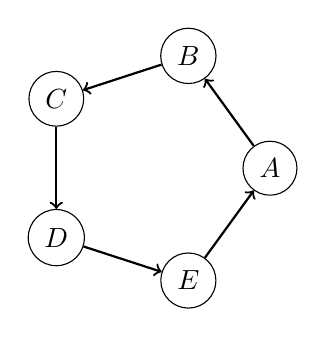
\begin{tikzpicture}
        \node[draw, circle] (a) at (0:1.5) {$A$};
        \node[draw, circle] (b) at (72:1.5) {$B$};
        \node[draw, circle] (c) at (144:1.5) {$C$};
        \node[draw, circle] (d) at (216:1.5) {$D$};
        \node[draw, circle] (e) at (288:1.5) {$E$};
        \draw[thick,->] (a) -- (b);
        \draw[thick,->] (b) -- (c);
        \draw[thick,->] (c) -- (d);
        \draw[thick,->] (d) -- (e);
        \draw[thick,->] (e) -- (a);
    \end{tikzpicture}
    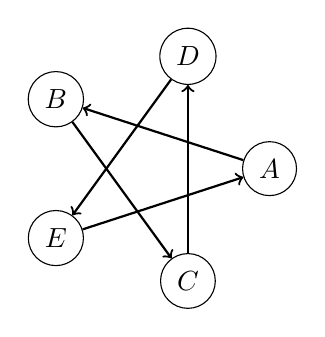
\begin{tikzpicture}
        \node[draw, circle] (a) at (0:1.5) {$A$};
        \node[draw, circle] (b) at (144:1.5) {$B$};
        \node[draw, circle] (c) at (288:1.5) {$C$};
        \node[draw, circle] (d) at (72:1.5) {$D$};
        \node[draw, circle] (e) at (216:1.5) {$E$};
        \draw[thick,->] (a) -- (b);
        \draw[thick,->] (b) -- (c);
        \draw[thick,->] (c) -- (d);
        \draw[thick,->] (d) -- (e);
        \draw[thick,->] (e) -- (a);
    \end{tikzpicture}
    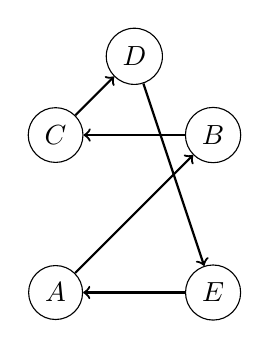
\begin{tikzpicture}
        \node[draw, circle] (a) at (0,0) {$A$};
        \node[draw, circle] (b) at (2,2) {$B$};
        \node[draw, circle] (c) at (0,2) {$C$};
        \node[draw, circle] (d) at (1,3) {$D$};
        \node[draw, circle] (e) at (2,0) {$E$};
        \draw[thick,->] (a) -- (b);
        \draw[thick,->] (b) -- (c);
        \draw[thick,->] (c) -- (d);
        \draw[thick,->] (d) -- (e);
        \draw[thick,->] (e) -- (a);
    \end{tikzpicture}
\end{frame}

\begin{frame}{Planar graphs}
    \begin{itemize}
        \pause\item A graph is \textbf{planar} if it can be drawn with no overlapping edges
        \pause\item A region enclosed by edges is called a \textbf{faces}
        \pause\item A connected planar graph obeys \textbf{Euler's formula}:
            $$ n_{\text{nodes}} - n_{\text{edges}} + n_{\text{faces}} = 2 $$
    \end{itemize}
\end{frame}

\begin{frame}{Trees}
	\begin{columns}
		\pause
		\begin{column}{0.3\textwidth}
			\includegraphics[width=\textwidth]{tree2}
			\par
			\vspace{2ex}
			\includegraphics[width=\textwidth]{tree}
		\end{column}
		\begin{column}{0.68\textwidth}
			\begin{itemize}
				\pause\item A \textbf{tree} is a special type of directed graph where:
					\begin{itemize}
						\pause\item One node (the \textbf{root}) has no incoming edges
						\pause\item All other nodes have exactly 1 incoming edge
					\end{itemize}
				\pause\item Edges go from \textbf{parent} to \textbf{child}
					\begin{itemize}
						\pause\item All nodes except the root have exactly one parent
						\pause\item Nodes can have 0, 1 or many children
					\end{itemize}
				\pause\item Used to model \textbf{hierarchies} (e.g.\ file systems, object inheritance, scene graphs, state-action trees, ...)
			\end{itemize}
		\end{column}
	\end{columns}
\end{frame}

\begin{frame}{Implementing trees}
	\begin{itemize}
		\pause\item A graph has a \textbf{root node}
		\pause\item Each node has a \textbf{collection of children}
		\pause\item Each node other than the root has a \textbf{single parent}
	\end{itemize}
\end{frame}

%\input{graph_traversal}
%\part{Linked lists}
\frame{\partpage}

\begin{frame}{Linked list}
	\begin{itemize}
		\pause\item Composed of a number of \textbf{nodes}
		\pause\item Each node contains:
			\begin{itemize}
		 		\pause\item An \textbf{item} --- the actual data to be stored
		 		\pause\item A pointer or reference to the \textbf{previous node} in the list (null for the first item)
		 		\pause\item A pointer or reference to the \textbf{next node} in the list (null for the last item)
			\end{itemize}
	\end{itemize}
	\pause
	\vspace{2ex}
	\begin{center}
	    \setlength{\tabcolsep}{0.2em}
		\begin{tabular}{|c|c|c|}
			\hline
			{\tiny prev} & {\tiny item} & {\tiny next} \\
			$\times$ & \texttt{\footnotesize first} & \tikzmark{nexta} \\\hline
		\end{tabular}
		\qquad
		\begin{tabular}{|c|c|c|}
			\hline
			{\tiny prev} & {\tiny item} & {\tiny next} \\
			\tikzmark{prevb} & \texttt{\footnotesize second} & \tikzmark{nextb} \\\hline
		\end{tabular}
		\qquad
		\begin{tabular}{|c|c|c|}
			\hline
			{\tiny prev} & {\tiny item} & {\tiny next} \\
			\tikzmark{prevc} & \texttt{\footnotesize third} & $\times$ \\\hline
		\end{tabular}
		
\begin{tikzpicture}
			[
			  remember picture,
			  overlay,
			  -latex,
			  yshift=0.5ex,
			  shorten >=1pt,
			  shorten <=1pt,
			]
			\draw ($ ({pic cs:nexta}) + (0, 0.5ex) $) to ($ ({pic cs:prevb}) + (-1.2ex, 0.5ex) $);
			\draw ($ ({pic cs:nextb}) + (0, 0.5ex) $) to ($ ({pic cs:prevc}) + (-1.2ex, 0.5ex) $);
			\draw ($ ({pic cs:prevb}) + (0, -0.5ex) $) to ($ ({pic cs:nexta}) + (1.2ex, -0.5ex) $);
			\draw ($ ({pic cs:prevc}) + (0, -0.5ex) $) to ($ ({pic cs:nextb}) + (1.2ex, -0.5ex) $);
		\end{tikzpicture}
	\end{center}
	\begin{itemize}
		\pause\item In C\#: \lstinline{LinkedList<ElementType>}
	\end{itemize}
\end{frame}

\newcommand{\footnoteref}[1]{$^{\text{\ref{#1}}}$}

\begin{frame}{Linked lists vs arrays}
	\begin{center}
		\begin{tabular}{|r|l|l|}
			\hline
			\textbf{Operation} & \textbf{Array} & \textbf{Linked list} \\\hline
			\pause Append & $O(1)$ & $O(1)$ \footnote{\label{f:llend}If we already have a reference to the last node} \\
			\pause Pop & $O(1)$ & $O(1)$ \footnoteref{f:llend} \\
			\pause Index lookup & $O(1)$ & $O(n)$ \\
			\pause Count elements & $O(1)$ & $O(n)$ \\
			\pause Insert & $O(n)$ & $O(1)$ \footnote{\label{f:llinsert}If we already have a reference to the relevant node} \\
			\pause Delete & $O(n)$ & $O(1)$ \footnoteref{f:llinsert} \\
			\hline
		\end{tabular}
	\end{center}
\end{frame}


\end{document}
